%% content.tex
%%

\chapter{Status Quo}
In diesem Kapitel wollen wir den aktuellen Stand der Wissenschaft vorstellen. Hierbei beziehen wir uns auf das Thema Lernen und Online-Hilfe. Welches Wissen gibt es hierbei bereits und auf welchem Stand sind diese? Das wollen wir in diesem Kapitel klären, bevor es zu den Grundlagen dieser Arbeit kommt

\section{Lernen}
Das Thema Lernen ist ein wichtiger Bestandteil dieser Arbeit. Aus diesem Grund wollen wir uns bevor wir unsere Problemstellung einsteigen mit dem aktuellen Stand des Lernens befassen und den aktuellen Stand der Forschung zum Thema Lernen aufzeigen mit unseren in der Arbeit verwendeten Konzepten.


\subsection{Problembasiertes Lernen}
">Problem based Lerning (PBL) is a learner-centred approach for designing learning environments in authentic, ill-structured problems"< entnommen aus \cite{zumbachproblembasiertes}. \par

Das Problembasierte Lernen, wie im Zitat deutlich wird, bezieht sich auf das Erarbeiten von selbstständigen Lösungsansätzen zum Lösen eines Problems. Der Lernende soll ein Thema selbstständig erarbeiten, ohne das jemand anderes einen Lösungsweg vorzeichnet. Auf dem Weg zu der Lösung eines Problems muss er evtl. mehrere Ansätze probieren um sein Ziel zu erreichen. Wie im Zitat bereits erwähnt steht der Lernende im Mittelpunkt. Der Lernende muss hierbei selbst die Initiative ergreifen. Ein Lehrer steht beim Lernprozess nur als Helfende Hand zur Seite. Er dient dabei lediglich als Coach, der evtl. aufkommende Fragen des Lernenden beantwortet und ihn in eine spezielle Richtung leitet, falls der Lernende nicht mehr weiterkommt. Beim Thema Software haben wir eine ähnliche Problemstellung. Ein möglicher Anwender kommt an einem Punkt in der Software nicht mehr weiter und muss selbstständig eine Lösung für das konkrete Problem finden. 
 
\subsection{Differenzielles Lernen}
Ein weitere Ansatz zum Thema Lernen gibt es in der Sporttheorie. Die Idee des differenziellen Lernens bezieht sich auf das Erlernen von Bewegungen im Sport. Beim differenziellen Lernen werden Bewegungen variiert. Beim Tischtennis beispielsweise wird ein Schlag auf verschiedene Wege durchgeführt. Hierbei werden vor allem Körperwinkel variiert. \footnote{Quelle: \cite{differenziellesLernen}} Es werden drei Bälle vom Lernenden gespielt und jede Bewegung sollte hierbei auf einem anderen Weg durchgeführt werden. Das Ziel dieser Form von Lernen ist es kein ideales Technikleitbild für eine Bewegung vorzugeben, also keine Lösung sondern die Bewegung so vielfältig wie möglich zu streuen. Wenn er dieses Training durchführt, dann kann ein Lernender in jeder Situation die korrekte Bewegung anwenden. Diese Form des Bewegungslernens ist sehr stark verwandt mit dem problembasierten Ansatz. Das Differenzielle Lernen gibt ebenfalls ein Problemstellung vor, die mit verschiedenen Lösungswegen gelöst werden soll. Der Unterschied hierbei besteht in der Vorgabe von Lösungsansätzen im Vergleich zum komplett selbständigen problematisierten Lernen.  Diese beiden Konzepte des Lernens wollen wir in dieser Arbeit für unsere Empfehlung verwenden.


\chapter{Grundlagen}
Um ein besseres Verständnis dieser Arbeit zu gewährleisten, sind gewisse Grundlagen zu dem Thema erforderlich. Diese Begriffe werden nachfolgend noch einmal aufgeführt, definiert und in den Zusammenhang mit dieser Arbeit gesetzt. Beginnen möchten wir dabei mit dem Ersten der vier Begriffe, nämlich der Online-Lernhilfe.
\section{Online-Lernhilfe}
Wir werden eine kurze Begriffsdefinition geben und anschließend die Verwendung in unserer Arbeit erläutern. Dies hilft beim Verständnis des Problems.
\subsection{Begriffsdefinition}
Die Online-Lernhilfe setzt sich aus zwei Begriffen zusammen, der Online-Hilfe und der Lernhilfe. Die Online-Hilfe bezeichnet eine „\textit{Hilfefunktion, die nur über eine direkte Verbindung mit dem Internet genutzt werden kann}“ \cite{dud1}. Die Lernhilfe beschreibt eine „\textit{Hilfe, Mittel oder Anhaltspunkt beim Lernen von etwas}“ \cite{dud2}. Somit ist die Online-Lernhilfe ein Hilfe-, Mittel- oder Anhaltspunkt, der eine Verbindung mit dem Internet voraussetzt.

\subsection{Verwendung in der Arbeit}
Unter Online-Hilfen verstehen wir die klassischen Hilfsmodule von Software. Diese bietet dem Nutzer Hilfe zu einem bestimmten Themengebiet in der Software. Die klassische Form ist ein Handbuch das zu der Software beigelegt wird. Dieses Handbuch erklärt die Software mit ihren Funktionen. Früher waren die Handbücher sehr umfangreich, so dass man zuerst mehrere Seiten dieses Handbuch lesen musste, um die Software überhaupt erst verstehen zu können. Heutzutage sind die Benutzeroberflächen vereinfacht, so dass die Software im Idealfall selbsterklärend ist und keine weitere Hilfestellung notwendig. Das Software immer mehr Prozesse abbilden kann, wird die Komplexität einer Software jedoch immer zunehmen. Damit die Komplexität weiterhin von einem User bedient werden kann, muss er zum einen neue Bedienelemente einer Software lernen und zum Anderen eine schnelle Hilfe erhalten, wenn er an einem bestimmten Punkt in der Software nicht weiterkommt.

\section{Adaption}
\label{ch:Content1}
Wie aus dem Titel unserer Arbeit ersichtlich, benötigen wir eine Definition des Adaptions-Begriffs, um unsere Arbeitsgebiete klar abzugrenzen.

\subsection{Begriffserläuterung}
Unter dem Begriff Adaption, welcher von dem lateinischen Wort „\textit{adaptare}“ stammt und „\textit{anpassen}“ bzw. „\textit{passend}“ herrichten \cite{dud3} bedeutet, versteht man die Anpassung eines Objekts an einen Zweck. 

\section{Adaption an den Nutzer}
Der Begriff der Adaption ist sehr breit auf den Bereich Online-Lernhilfe anwendbar. Eine Adaption ist deshalb an sehr vielen Stellen möglich. Aus diesem Grund wurde in Absprache mit den Betreuern festgestellt, dass die Lösungsvorschläge nur eine Adaption an den Nutzer beinhalten sollen.Eine Adaption an verschiedene Endgeräte, wie Tablets, Smartphones oder Computer sollen deshalb aus der Betrachtung und Bewertung ausgeschlossen werden. Lösungsvorschläge, welche im Verlauf der Arbeit vorgestellt werden und adaptiv sind, stellen folglich ausschließlich eine Anpassung an den Nutzer dar. Darunter kann man sich zum Beispiel einen grafisch aufgearbeiteten Hilfetext für den Benutzer der Software vorstellen, der sich dynamisch an den derzeit verwendeten Teil der Software anpasst.

\section{Gamification}
Als zweite Grundlage haben wir den Ansatz Gamification. Dieser ist für unsere Erläuterung sehr wichtig und wird deshalb im Folgenden aufgeführt.
\subsection{Definition}
„\textit{Gamification ist die Übertragung von spieltypischen Elementen und Vorgängen in spielfremde Zusammenhänge mit dem Ziel der Verhaltensänderung und Motivationssteigerung bei Anwenderinnen und Anwendern. Zu den spieltypischen Elementen gehören Beschreibungen (Ziele, Beteiligte, Regeln, Möglichkeiten), Punkte, Preise und Vergleiche. Zu den spieltypischen Vorgängen zählt die Bewältigung von Aufgaben durch individuelle oder kollaborative Leistungen.}“ \cite{gamification}

\subsection{Verwendung in unserer Arbeit}
Da es sich bei unseren Lösungsvorschlägen hauptsächlich um verschiedene Arten von Hilfen für ein konkretes Problem handelt, verwenden wir nur einen Teil aus dem Bereich des Gamification in unseren Lösungsvorschlägen. Es handelt sich bei dem verwendeten Teil um die spieltypischen Elemente, wie Punkte, Preise und Vergleiche und die spieltypischen Vorgänge. Wie diese dann konkret in unseren Lösungsvorschlägen verwendet werden, lässt sich im Kapitel der Lern-App nachlesen.

\section{Recommendersysteme}
Ein Teil unseres Lösungsansätzes verwendet ein Recommendersystem.
\subsection{Begriffserläuterung}
„\textit{Ein Recommendersystem sammelt Empfehlungen von Benutzern, aggregiert diese Empfehlungen und leitet sie an geeignete Adressaten weiter.}“(aus \cite{recommender})

\subsection{Verwendung in unserer Arbeit}
In unserer Arbeit wollen wir die Recommendersysteme in Form eines Expertensystems verwenden.  Der Experte kennt ein bestimmtes Gebiet der Software und generiert später die Empfehlung. Diese kann im Kontext des Lernens entweder ein Tipp zur Lösungsfindung sein oder aber auch die direkte Lösung zu einem Problem. Im Softwareumfeld kann dies besser differenziert werden. Entweder der Experte zeigt einen möglichen  Weg auf um das Problem zu beseitigen oder aber er erarbeitet mit dem Lernenden zusammen als Coach die Lösung des Problems. Diese beiden Möglichkeiten können mithilfe eines Recommendersystems begangen werden und werden in unserem dritten Lösungsansatz weiter vertieft.






%% ===========================
\chapter{Nutzer}
Da unsere Arbeit die Adaption auf den Nutzer bezieht, müssen wir zuerst klären, welcher konkrete Nutzer bei unserer Arbeit in Frage kommt. Hierzu wollen wir die einzelnen Nutzerrollen der Zielsoftware mit deren Charakteristika vorstellen.


\section{Nutzerrollen}
Das Anwendungsfeld der Software ist wie in Einleitung beschrieben eine Hochschule. Im Mittelpunkt der Anwendung steht der Student, der sozusagen der Endkunde ist. Alle Dienstleistungen, die von der Software übernommen werden sind für den Studenten. Hierbei werden verschiedene Prozesse durchlaufen, die von verschiedenen Personen während des sogenannten Studen-Lifecycles gesteuert werden. Im folgenden werden wir erklären, wie die gegebene Nutzerrolle die Zielsoftware verwendet und welche Ziele er bei der Verwendung verfolgt.
\subsection{Professoren}
Beginnen wollen wir mit der Persona Professor. Er ist für die Lerninhaltsaufbereitung des Studenten zuständig. Ein Professor hat eher weniger mit der Software zu tun, da die meiste Arbeit die Sekretärin abnimmt. Die Verwendung beschränkt sich auf das Lesen eines Termines oder das Eintragen einer Lehrveranstaltung. Weiterhin auf ein eventuelles Einladungsmanagement. Ein Professor ist somit ein Nutzer, der sehr wenig Zeit mit der Verwendung der Software aufbringt. Somit muss er, wenn er in einem Problem bei der Verwendung der Software steckt schnell eine Lösung haben. Weiterhin ist die Zeit des Professors aufgrund seiner Aufgabengebiete begrenzt, womit eine lange Einarbeitungszeit ebenfalls vermieden werden sollte.
\subsection{Studenten}
Die Studenten sind wie Eingangs erwähnt die Profiteure der Software. Dadurch, dass alle Prozesse, die von der Software abgebildet werden nur für den Studenten da sind, steht er im Fokus. Die Verwendung der Software hält sich allerdings vom zeitlichen Aufwand her im Rahmen. Er verwendet zwar viele Bereiche der Software allerdings nur sehr kurz und schnell. Sein primäres Ziel bei der Verwendung ist Ähnlich dem Professor. Er möchte schnell an Informationen kommen und sich nicht lange in eine Software einarbeiten, da er andere Inhalte für sein Studium lernen muss. Somit sollte er komplizierte Lerninhalte einfach aufbereitet bekommen, so dass er schnell ein gutes Verständnis erlangen kann.

\subsection{Studierendensekretariat}
Das Studierendensekretariat oder auch Help-Desk genannt ist für die komplette Verwaltungsarbeit eines Studenten zuständig. Die Nutzer dieser Rolle verwenden die Software im täglichen Gebrauch und dies für mehrere Stunden am Tag. Aus diesem Grund müssen sie die Software möglichste effektiv und schnell beherrschen. Komplexe Prozesse bei der Bedienung der Software muss den Arbeitern geläufig sein, um effizient arbeiten zu können. Weiterhin muss bei einem konkreten Problem beim Verwenden der Software schnell Abhilfe geschaffen werden. 
\subsection{Studiengangsbearbeiter}
Eine besondere Rolle im Lebenszyklus der Software nimmt die Rolle des Studiengangsbearbeiters ein. Diese ist für die Modellierung von Studiengängen zuständig. Diese Art von Nutzer verwenden die Software sehr intensiv und müssen sehr effizient arbeiten, da sie die Software jeden Tag intensiv mit vielen Inhalten nutzen. Die Modellierungsinhalte, welche mit der Software getätigt werden sind sehr komplex und erfordern ein hohes Maß an Konzentration. Damit man diesen Wünschen gerecht werden kann, muss unsere Lösung viel Lerninhalt in kurzer Zeit aufbereiten und für den Nutzer sinnvoll erklären. Natürlich kann die Hilfe nur einen kleinen Teil der Inhalte lernen. Die Basis sollte weiterhin eine intensive Schulung sein, bevor der Nutzer die Software verwendet. Die adaptive Online-Lernhilfe sollte den Nutzer bei der Lösungsfindung in diesem Fall unterstützen und ihm helfen, die Inhalte der Schulung evtl. nachträglich noch einmal zu wiederholen und zu vertiefen.

\subsection{Admins}
Eine weitere Rolle, die nicht missachtet werden sollte sind die Administratoren der Software. Diese sind für die Konfiguration der einzelnen Bereiche in der Software zuständig und normalerweise erster Ansprechpartner, wenn Probleme bei der Verwendung der Software auftreten. Der Admin muss normalerweise entscheiden, ob es ein Software-Fehler ist oder ein anderes Problem besteht. Bei kleineren Hochschulen kann diese Rolle auch wegfallen, da nicht genügend Kapital für die Finanzierung einer solchen Stelle vorhanden ist. Da die Zielsoftware für größere Hochschulen mit teils sehr technischen Schwerpunkten (Informatik, Maschinenbau, etc.) konzipiert ist, ist anzunehmen, dass es gesonderte Stellen zur Administration der Software gibt. Die Schwerpunkte hier beim eigentlichen Verwenden der Software liegen in dem Deployment von Updates oder dem Lösen von Konfigurationsproblemen. Für diese Zielgruppe soll das Hilfesystem vorwiegend schnell Informationen bereitstellen, so dass der Admin unverzüglich weiterarbeiten kann.

\section{Nutzer Klassifizierung}
Nachdem die einzelnen Nutzerrollen vorgestellt wurden, werden wir eine Klassifizierung vornehmen um für die klassifizierten Nutzergruppen die passenden Lösungsansätze vorstellen zu können. Die Klassifizierung erfolgte anhand der in Abbildung \ref{img1:userRoles} sichtbaren Kriterien: Nutzunghäufigkeit (Powernutzer, Gelegenheitsnutzer) und Art der Nutzung (effektive Nutzer, informationsorientierte Nutzer und schnelle Nutzung). Diese Kriterien haben wir den jeweiligen Rollen zugeordnet. Durch die Verknüpfung in einem ungerichteten Graphen sind wir zu der Nutzerklassifizierung gekommen. Die Nutzerklassen werden wir im folgenden erläutern.
\begin{figure}[ht]
\begin{center}
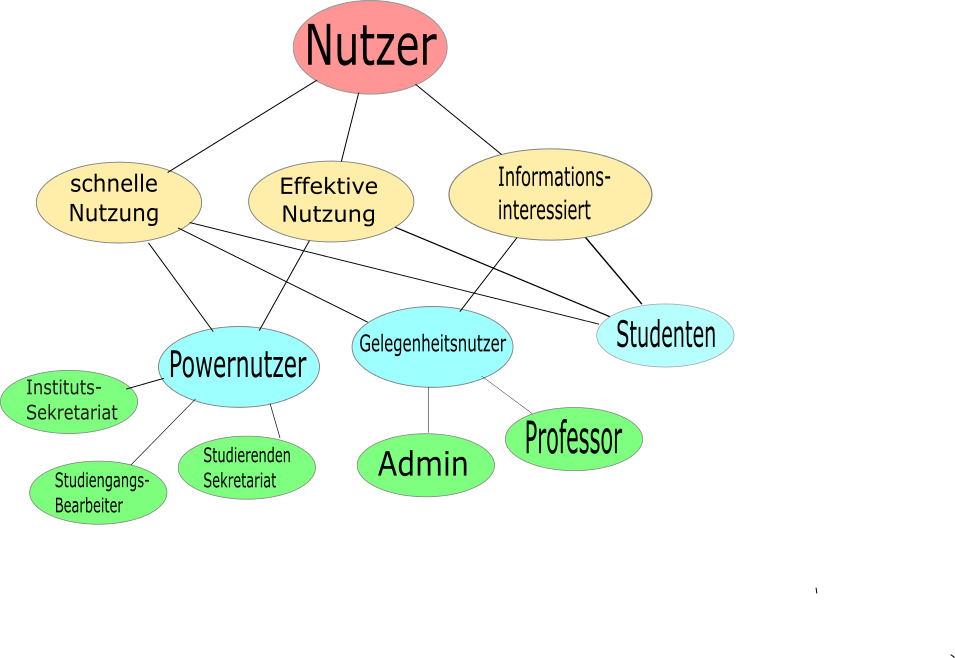
\includegraphics[width = 0.95\textwidth]{Nutzerrollen.png}
\caption{Nutzerrollen mit einer Bewertung anhand von Kriterien}
\label{img1:userRoles}
\end{center}
\end{figure} 

\subsection{Lösungsorientierte Nutzer}
Der lösungsorientierte Nutzer möchte schnell die Lösung zu seinem aktuellen Problem haben. Er möchte sich nicht lange mit Online-Hilfesystemen oder langen Suchen beschäftigen. Zu dieser Gruppe gehören vor allem die Gelegenheitsnutzer. Diese verwenden die Software selten und sind deshalb wenig angetan, wenn sie lange in einem bestimmten Problem stecken. Ihnen muss schnell geholfen werden, so dass kein Frust beim Verwenden der Software aufkommt. Hier läuft die Lösung nach dem Prinzip ab, dass ein Problem beim Verwenden der Software auftritt und schnellstmöglich eine Lösung her muss. 
\subsection{Powernutzer}
Diese Nutzergruppe verwendet die Software meist jeden Tag und dies mehrere Stunden täglich. Dies bedeutet es müssen sehr viele Inhalte gelernt werden. Wenn möglich in möglichst kurzer Zeit. Dies erfordert ein Lernen von mehreren Wegen zur Lösung des Problems. Für diese Art von Nutzern zählt eine effektive Nutzung der Software. Die Lerninhalte müssen somit möglichst umfassend sein und entsprechend aufbereitet werden. 
\subsection{Studenten}
Die Studenten erhalten bei uns eine extra Klasse. Sie setzen die Software sehr sporadisch ein und möchten nicht viel neue Inhalte lernen, da sie schon mit anderen Themen ihres Studiums sehr beschäftigt sind. Wenn sie die Software verwenden, dann möchten sie nicht viel neue Inhalte lernen. Wenn überhaupt, dann mit Spaß verbunden. Sie benötigen somit eine extra Motivation um neue Inhalte der Software zu lernen. Weiterhin schwierig bei dieser Nutzergruppe ist die Diversität der Nutzertypen. Dies bedeutet, dass viele verschiedene Fachbereiche, von sehr technisch versierten Leuten wie Ingenieursstudiengänge bis stark intellektuelle Studiengänge wie Germanistik oder Jura bedient werden müssen. Diese starke Diversität veranlasst uns die Gruppe der Studenten als extra Klasse zu betrachten. 


%% content.tex
%%

%% ==============
\chapter{Lösungsansätze}
Dieses Kapitel widmet sich den Lösungsansätzen, die als Grundlage für unsere abschließende Empfehlung dienen. Es handelt sich dabei um verschiedene Ansätze, die aufgrund unserer Nutzerklassifizierung und deren Ziele entstanden sind.
\section{Klassische Hilfe}
Das klassische Hilfesystem soll unserer Klasse der Problemorientierten Nutzer weiterhelfen. Durch eine schnelle Lösungsfindung und Aufbereitung soll dem Nutzer geholfen werden.

\begin{figure}[ht]
\begin{center}
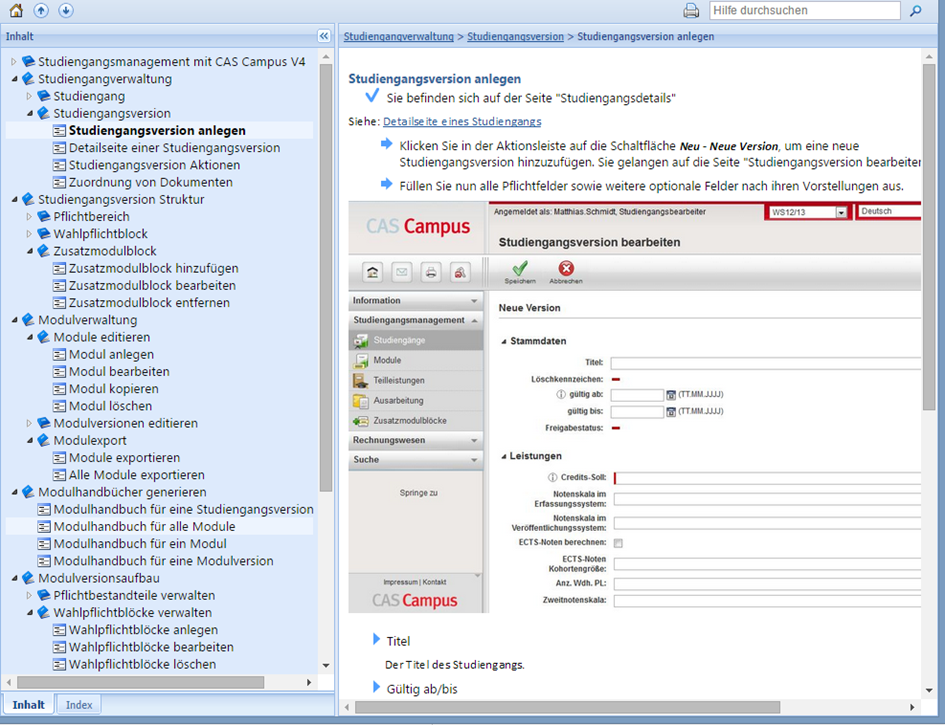
\includegraphics[width = 0.95\textwidth]{onlineHilfe.png}
\caption{Klassischer Aufbau eines Hilfesystems}
\label{img1:userRoles}
\end{center}
\end{figure} 
\subsection{Erläuterung}
Die klassische Hilfe entspricht, wie der Name bereits vermuten lässt, einem Hilfesystem wie man es bereits aus mehreren Programmen kennt. Ein Hilfesystem ist die „\textit{Gesamtheit an Informationen, die gegeben werden, um dem Benutzer beim Umgang mit [Anwendungs]programmen zu helfen}“ (Duden, 2015). Es handelt sich im Falle der Abbildung um ein Handbuch welches online abgerufen werden kann. Der Inhalt der Hilfe wird als grafisch aufbereiteter Text dargestellt und mit Bildausschnitten aus dem Programm ergänzt. Die aufgerufene Hilfeseite wird wie in Abbildung \ref{img2:helpSystem} auf der rechten Seite des Fensters dargestellt. Die linke Seite des Fensters enthält die einzelnen Hilfeseiten, nach Inhalt in diverse Kategorien geordnet. Eine Indexierung der Hilfeseiten ist ebenfalls vorhanden und lässt sich über einen weitere Registerkarte im linken Bereich einblenden. Die Suchfunktion nach Inhalt oder Indexeinträgen befindet sich in der Kopfzeile des Fensters. Diese Form der Hilfe bietet die Möglichkeit zu einem konkreten Problem die genaue Lösung zu erhalten.

\section{Lernspiel-App}
Der zweite Lösungsansatz soll eine Lösung in Form einer sogenannten Lernspiel-App aufzeigen. Zuerst wird eine Begriffsdefinition von App durchgeführt bevor die konkrete Lösung vorgestellt wird.

\subsection{App}
Der App-Begriff bezieht sich in unserer Arbeit auf einen kleinen Prozess, der mit einer Software durchgeführt werden kann. Dieses Prinzip kann man am Besten anhand von Unix-Systemen erklären. Hier gibt es für jedes kleine Teilproblem, welches bei der Verwendung eines Computers eintritt ein extra Programm. Dieses Programm macht genau die Aufgabe, die es soll und keine zusätzlichen Extra-Funktionen. Ein gutes Beispiel ist ein Texteditor. Bei einer grafischen Oberfläche beherrscht dieser beispielsweise die Funktion suchen und ersetzen. Weiterhin kann der Editor beispielsweise bestimmte Textfelder rot markieren und eine Datei von dem geschriebenen anlegen. In einer Unix-Konsole gäbe es für alle diese Funktionen einen extra Befehl, der genau diese eine Funktion erfüllt. Dies hat den Vorteil, dass sehr effizient gearbeitet werden kann. Dieses Prinzip verwenden die modernen Apps auf dem Smartphone ebenfalls. Für jeden Anwendungsfall gibt es genau eine App. Das Smartphone besitzt somit eine Ansammlung mehrerer Apps zur Lösung von mehreren Teilproblemen. Eine solche Plattform ist in Abbildung \ref{img1:smartDesign} abgebildet. Auf der linken Seite befinden sich die Icons von mehreren Apps. Auf der rechten Seite ist der konkrete Prozessworkflow, in diesem Beispiel eine Kontaktliste sichtbar. 
\begin{figure}[ht]
\begin{center}
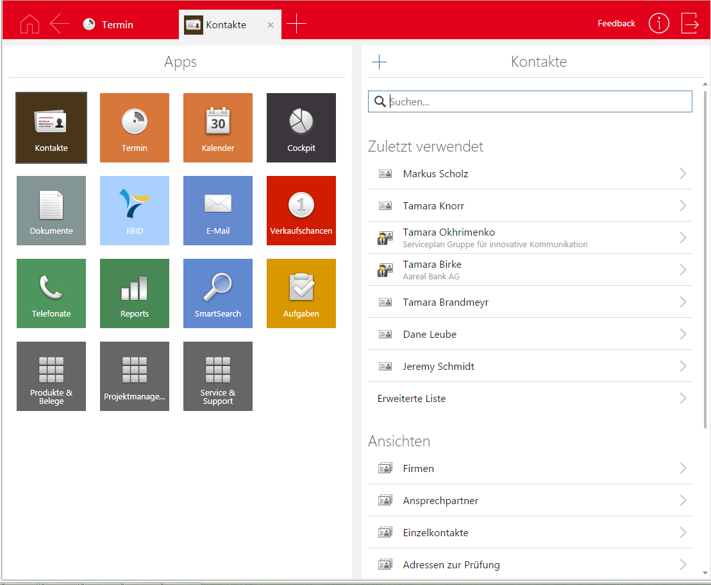
\includegraphics[width = 0.95\textwidth]{smartDesign.png}
\caption{App-Plattform und Prozessworkflow einer App}
\label{img1:smartDesign}
\end{center}
\end{figure} 

\subsection{Lernspiel}
Unter einem Lernspiel verstehen wir die Verknüpfung von Gamification-Ansätzen mit dem Erlernen von neuen Inhalten. Hier sind Konzepte für ein umfangreiches Belohnungssystem von Interesse. Ein Nutzer kann eine Belohnung erhalten wenn er eine bestimmte Aufgabe lösen kann. Diese Aufgabe bezieht sich immer auf das Software-Feld. Hierzu erhält der Nutzer ein gezieltes Problem, welches er eventuell auf verschiedenen Wegen lösen kann. Dieser Prozess des Lernens soll durch eine Belohnung am Ende motiviert werden. Erreicht der Nutzer ein bestimmtes Lernziel, so erhält er beispielsweise einen sogenannten Badge (kleine Auszeichnung) oder erreicht das nächste Level, wo ihm ein komplexeres Problem erwartet. 

\subsection{Lösungsansatz}
Die Verbindung vom App-Prinzip mit dem Lernspiel soll unser zweiter Lösungsansatz repräsentieren. Das daraus folgende Konzept soll eine App designen, die komplexe Inhalte unserer Software in einem Spiel aufbereitet. Dieses Spiel besteht aus mehreren Leveln, die unterschiedliche Komplexitätsgrade beherbergen. Der Schwierigkeitsgrad der Lernspiel-App hängt von den Erfahrungen des Nutzers ab, der das Spiel durchführt. Wenn keine Erfahrungen von seitens des Nutzers bestehen, so fängt er bei der einfachsten Problemstellung an und arbeitet sich durch mehrere Levels. Hierbei muss aufgepasst werden, dass der ganze Ansatz nicht zu verspielt ist, da die problembasierten Nutzer sich nicht lange mit so einem simplen Spiel aufhalten wollen. Für die Studentengruppe hingegen soll der Spaß im Vordergrund stehen weshalb eine spannende Aufbereitung der Inhalte wichtig ist. Damit die effektiven Nutzer bedient werden können, muss die Lernspiel-App viele Problemstellungen innerhalb der Software behandeln und möglichst viele Levels anbieten.


\section{Expertensystem}
Unser sogenanntes Expertensystem beruht auf einem Recommendersystem. Es soll, wie in einem Recommender, Empfehlungen von Nutzern generieren. Diese Empfehlungen werden direkt von einem Nutzer zum Nächsten weitergegeben. Wichtig hierbei ist die Identifikation des Experten der die Empfehlungen abgibt. Diese Identifikation soll anhand der Lernspiel-App erfolgen. Wer hier gut abschneidet, also eine schnelle und effektive Lösung für das gestellte Problem findet, der kann sich durch Badges einen Expertenstatus erarbeiten. Dieser Status gilt immer für einen bestimmten Bereich der Software, also einer App und einem dazugehörigen Workflow. Der Lösungsansatz muss die Information, wer ein solcher Experte für einen bestimmten Bereich ist, bereitstellen. Unsere Recommender-Empfehlung besteht aus der Anzeige eines Experten für einen bestimmten Bereich innerhalb der Software. Aufgrund dieser Anzeige kann ein Nutzer, der gerade Hilfe benötigt den Experten identifizieren und ihn um Rat bitten. Diese Frage kann er dann entweder per E-Mail oder direkt per Telefon durchführen. Eine weitere Möglichkeit zum Erlangen des Expertenstatus kann durch das Manuelle Einstellen durch einen Administrator sein, der im Backend dies einstellt.


\chapter{Empfehlung}
Unsere abschließende Empfehlung soll die Lösungsansätze anhand der Nutzerklassen und unserer Kriterien bewerten. Hierzu erfolgt jeweils eine Gegenüberstellung.
\section{Bewertung der Lösungsansätze anhand der Nutzerklassen}
\section{Bewertung der Lösungsansätze anhand der Kriterien}

\section{Konkrete Empfehlung}

\chapter{Zusammenfassung}
Die Aufgabe dieser Seminararbeit war es, ein adaptives Online-Hilfesystem zu entwickelt. Gestartet haben wir mit der Frage nach der Adaption. Hier haben wir uns, durch die Vorgabe unserer Betreuer, auf die Adaption an den Nutzer konzentriert. Nachdem wir alle Nutzerrollen aufgezeigt haben, konnten wir eine Klassifizierung der Nutzer durchführen. Diese Klassifizierung hat uns geholfen auf den Nutzer passende Lösungsansätze zu entwickeln. Diese sind durch verschiedene Grundlagen des problembasierten und differenziellen Lernens entstanden. Weiterhin konnten wichtige Ansätze der Gamification in einer App-Lösung erarbeitet werden. Eine weitere Lösung ist durch eine Recommendersystem-Grundlage entstanden. Damit ein besserer Vergleich stattfinden konnte, wurde die bisherige Lösung eines klassischen Hilfesystems vorgestellt. In der folgenden Gegenüberstellung der Lösungsansätze wurden die Lösungen zuerst mit den Nutzerklassen und anschließend nach unseren selbst auferlegten Kriterien bewertet. Die daraus folgende Bewertung hat gezeigt, dass eine Kombination von allen drei Lösungsansätzen sinnvoll ist und durchgeführt werden kann.

\subsection{Ausblick}
Für eine konkrete Ausarbeitung unserer Empfehlung ist eine Ausarbeitung eines Konzeptes basierend auf unseren Lösungsansätzen der nächste Schritt. Die aufgezeigten Konzepte sollen hierbei in einen konkreten Software-Workflow implementiert werden, so dass eine Lernspiel-App entstehen kann. Das Ziel dieser App soll es sein, die Nutzer zu schulen und ihnen neue Lerninhalte der Software zu vermitteln. Weiterhin sollen, darauf aufbauend, führende Experten identifiziert werden, die anderen Nutzern bei konkreten Problemen bei der Verwendung der Software schnell weiterhelfen können.


